%  dvips -t letter specfem.dvi -o specfem.ps ; ps2pdf specfem.ps
%  pdflatex specfem.tex

\documentclass[10pt,fleqn,letterpaper]{article}

\usepackage{amsmath}
\usepackage{amssymb}
\usepackage[round]{natbib}
\usepackage{xspace}
\usepackage{graphicx}
\usepackage{xcolor,listings}
%\usepackage[space]{accsupp}

% For nice menu descriptions
\IfFileExists{menukeys.sty}{
\usepackage[mackeys=text]{menukeys}
}{
\newcommand{\keys}[1]{\texttt{##1}}
\newcommand{\menu}[1]{\texttt{##1}}
\newcommand{\cmd}{command}
\newcommand{\ctrl}{control}
\newcommand{\Alt}{alt}
}

%\usepackage{fancyhdr}
%\pagestyle{fancy}

%=====================================================
%       SPACING COMMANDS (Latex Companion, p. 52)
%=====================================================

\usepackage{setspace}

\usepackage[margin=1in]{geometry}

%\include{NEWCOMMANDS}
\newcommand{\specfem}{\textsc{Specfem3D}}
\newcommand{\cubit}{\textsc{Cubit}}
\newcommand{\geocubit}{\textsc{GeoCubit}}
\newcommand{\paraview}{\textsc{Paraview}}
\newcommand{\grace}{\textsc{Grace}}
\newcommand{\blue}[1]{\textcolor{blue}{#1}}


\graphicspath{
  {figures/}
}

\title{\specfem\ Tutorial for 2013 CIG-QUEST-IRIS Workshop}
\author{Carl, Qinya, Elliott, Emanuele}
\date{Last compiled: \today}

\usepackage[bookmarks=true,colorlinks=true,%
            pdfusetitle=true%
           ]{hyperref}

\definecolor{codebg}{RGB}{238,238,238}
\definecolor{codeframe}{RGB}{204,204,204}
\lstset{
  language=bash,
  basicstyle=\small\ttfamily,
  columns=fullflexible,
  keepspaces=true,
  breakatwhitespace=true,
  breaklines=true,
  prebreak=\raisebox{0ex}[0ex][0ex]{%
    \ensuremath{\backslash}},
%  postbreak=\raisebox{0ex}[0ex][0ex]{%
%    \BeginAccSupp{method=plain,ActualText={}}%
%      \textcolor{red}{\rotatebox[origin=c]{180}{$\Lsh$}}%
%    \EndAccSupp{}\space%
%  },
  backgroundcolor=\color{codebg},
  frame=single,
  framesep=10pt,
  rulecolor=\color{codeframe}
}

%=====================================================
\begin{document}
%=====================================================

\maketitle

%=====================================================

%\tableofcontents

\subsection*{Overview}

%--------------

\subsection*{Document Conventions}

\begin{enumerate}
\item In this document, commands you should run in your shell or code blocks
      you should edit are indicated by an framed grey box:
\begin{lstlisting}
This is a code block.
\end{lstlisting}

\item Things you should type at the prompt are prefixed by a dollar sign \$,
      and the output from commands is not. Comments are prefixed by a hash \#.
\begin{lstlisting}
$ echo "A command you can run" | sed 's/can/have/g' # This is a comment.
A command you have run
\end{lstlisting}

\item Lines that have been wrapped are indicated by the backslash~$\backslash$ at the
      end of the line and the symbol~\textcolor{red}{\rotatebox[origin=c]{180}{$\Lsh$}}
      at the beginning of the continued line. Most shells will understand the trailing
      backslash to indicate a continued command, so you should be able to copy all
      wrapped lines directly without any issues. Line breaks do not occur in the
      middle of words, so remember to include a space between each wrapped line if
      you are typing it out yourself.
\begin{lstlisting}
This is a very long line that will wrap because it goes on and on and on and also could be \
considered a run-on sentence, too.
\end{lstlisting}
\end{enumerate}

%--------------

\subsection*{Log-in instructions}

\begin{enumerate}
\item get account info from ARSC
\item ssh into ARSC (is X11 okay from mac? -X?)
\item Explain text editing (vi, gedit, emacs)
\end{enumerate}

%---------------

\subsection*{Step-by-step instructions, example 1: homogeneous halfspace synthetic seismograms (better call it forward simulation?)}

The purpose of this example is to step through all the key steps of \specfem: get the code, configure the code for your cluster, generate a mesh using (\textsc{Geo})\cubit, partition the mesh, generate databases, run the solver, and check the output. The example is trivial, but it is important to remember that 

\begin{enumerate}
\item Check what modules are loaded by default:
%
\begin{lstlisting}
$ module list
Currently Loaded Modulefiles:
  1) pgi/13.4                 3) netcdf/4.3.0.pgi-13.4
  2) openmpi-pgi-13.4/1.4.3   4) PrgEnv-pgi/13.4
\end{lstlisting}

If you do not see these modules listed, load the PGI compiler environment with \lstinline{module load PrgEnv-pgi}.

\item Change to the \verb+$CENTER+ directory (as \verb+$HOME+ has a limited quota of 4 GB), and check out two copies\footnote{There's no need for two copies, but they will make it a bit easier to keep track of the different exampled.} of the \specfem\ master branch from the code repository on GitHub (\url{https://github.com/geodynamics/specfem3d}) \blue{We will need to (a) pick a random revision (not recommended) or (b) tag a revision (more useful).}
%
\begin{lstlisting}
$ cd $CENTER
$ git clone --recursive https://github.com/geodynamics/specfem3d.git SPECFEM3D_default
$ git clone --recursive https://github.com/geodynamics/specfem3d.git SPECFEM3D_socal
\end{lstlisting}
%
(This may take a few minutes.)

\item check version info \blue{Commit ID will need to be fixed.}
%
\begin{lstlisting}
$ cd SPECFEM3D_default
$ git status
# On branch master
nothing to commit, working directory clean
$ git show
commit 846f6e400927b639d94bfba3a76ca132e07ef03e
Merge: 4ba0960 fa99f77
Author: Matthieu Lefebvre <ml15@princeton.edu>
Date:   Mon Dec 2 11:07:05 2013 -0800

    Merge pull request #74 from carltape/master

    added a clarification comment for running xcombine_vol_data after generating the databases.
\end{lstlisting}

The {\em base directory} for the code is \path{SPECFEM3D_default}, which we will call \path{SPECFEM3D} in the instructions.

\item Take a quick look at the user manual, mainly as a reminder to come back to it for details. 
%
\begin{lstlisting}
$ evince doc/USER_MANUAL/manual_SPECFEM3D_Cartesian.pdf &
\end{lstlisting}

\item Check that all software is available (or that modules are loaded):
\begin{lstlisting}
$ which mpirun # OpenMPI
$ which cubit  # Cubit
$ which python # Python
\end{lstlisting}

\item Configure package, using the Portland compiler, in our case:
\begin{lstlisting}
$ ./configure FC=pgf90 MPIFC=mpif90
\end{lstlisting}

If successful, this command will generate several \path{Makefile}s in the \path{SPECFEM3D} main directory, subdirectories of \path{src/}, as well as \path{shared/constants.h} and \path{shared/precision.h}, among others.

\item Adapt the run scripts for your cluster and your example.

- Copy run scripts from \path{utils/Cluster/} into \path{SPECFEM3D/}, e.g.,
\begin{lstlisting}
$ cd utils/Cluster/pbs/
$ cp go_decomposer_pbs.bash go_generate_databases_pbs.bash go_solver_pbs.bash ../../../
$ cd ../../../
\end{lstlisting}

For ARSC, set all bash scripts to run in the \texttt{standard} queue (the queue will depend on your specific cluster) by editing the line
\blue{(do we need to warn people to also delete one \# from the line of \#\#PBS -q debug?)}
\begin{lstlisting}
#PBS -q standard
\end{lstlisting}
(The default simulation time and number of cores is okay for this example.)
 
\item The rest of the instructions follow from the homogeneous halfspace example here
\begin{lstlisting}
SPECFEM3D/examples/homogeneous_halfspace/README
\end{lstlisting}

Copy the input files from examples directory into \path{SPECFEM3D/DATA/}
\begin{lstlisting}
$ cd examples/homogeneous_halfspace/
$ cp DATA/* ../../../DATA/
\end{lstlisting}
%
Note that only three input files are required: for the source (\path{CMTSOLUTION}), for the stations (\path{STATIONS}), and for the simulation parameters (\path{Par_file}).

\item Create mesh:

From the directory \path{SPECFEM3D/examples/homogeneous_halfspace}, open the \cubit\ GUI, \path{claro}:
\begin{lstlisting}
$ claro
\end{lstlisting}
\blue{maybe warn people that the X11 forwarding can be slow?}
%
(Close the ``Tip of the Day''.)
To ensure that the path is local and the needed python modules and scripts are accessible, \menu{File > Set Directory}, then click \menu{Choose} \blue{(Choose what? examples/homogenous\_halfspace/?)}, which is equivalent to typing in the \cubit\ command window \lstinline{cd 'examples/homogeneous_halfspace/'} (note the single quotes are required).

Run the meshing script: from the Menu bar, select \menu{Tools > Play Journal File}, set \menu{Files of Type} to \menu{All Files}, then select \path{block_mesh.py}.
\blue{cubit2specfem3D.py needs to be fixed!}

If everything goes fine, this script creates the ten mesh files in subdirectory \path{MESH/}:
\begin{lstlisting}
$ ls MESH
MESH/absorbing_surface_file_bottom
MESH/absorbing_surface_file_xmax
MESH/absorbing_surface_file_xmin
MESH/absorbing_surface_file_ymax
MESH/absorbing_surface_file_ymin
MESH/free_surface_file
MESH/materials_file
MESH/mesh_file
MESH/nodes_coords_file
MESH/nummaterial_velocity_file
\end{lstlisting}

You should be able to translate, rotate, and zoom on the mesh using a three-button mouse. (This can be emulated if you set X11 preferences, then (on a Mac) hold the \keys{\ctrl}, \keys{\Alt}, or \keys{\cmd} buttons while clicking and moving the mouse.)

The \cubit\ graphics window should show a mesh similar to that of Figure 1.
\begin{figure}[h]
\begin{center}
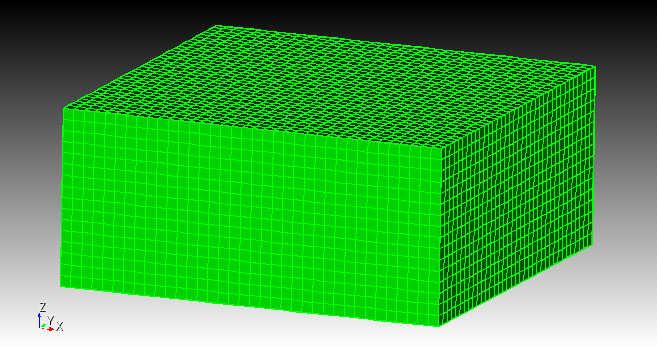
\includegraphics[width=0.7\textwidth]{picture_of_this_homogeneous_regular_mesh.png}
\end{center}
\caption{\cubit\ mesh for example 1}
\end{figure}

\item decompose mesh files:

Compile the decomposer in directory \path{SPECFEM3D/}:
\begin{lstlisting}
$ make xdecompose_mesh
\end{lstlisting}
%
This will compile the partitioner \textsc{Scotch}.

Then run the decomposer:
\begin{lstlisting}
$ qsub go_decomposer_pbs.bash
\end{lstlisting}
%
You can check the status of the job with the command
%
\begin{lstlisting}
$ qstat -u $USER
\end{lstlisting}
%
which should display something like:
%
\begin{lstlisting}
scyld: 
                                                               Req'd  Req'd      Elap
Job ID       Username Queue       Jobname       SessID NDS TSK Memory Time     S Time
------------ -------- ----------- ------------- ------ --- --- ------ -------- - ----
690722.scyld username standard_16 go_decomposer     --   1   1     -- 01:00:00 Q   -- 
\end{lstlisting}

The job should take about 20 seconds. As the job progresses, the \texttt{S} column will change from \texttt{Q(ueued)} to \texttt{R(unning)} to \texttt{C(ompleted)}. The process of the parallel job is summarized in \path{OUTPUT_FILES/jobid.scyld.o}. If successful, it creates the four mesh partitions \path{proc000***_Database} in the directory \path{OUTPUT_FILES/DATABASES_MPI/}. The output file \path{OUTPUT_FILES/*.o} contains information on the partitioning.

\item Generate databases:

Compile \path{xgenerate_databases} in the directory \path{SPECFEM3D/}:
\begin{lstlisting}
$ make xgenerate_databases
\end{lstlisting}
Submit the job:
\begin{lstlisting}
$ qsub go_generate_databases_pbs.bash
\end{lstlisting}

The job should take about a minute.
It creates binary mesh files, e.g. 
\begin{lstlisting}
proc000***_{rho,vp,vs,x,y,z,ibool,external_mesh}.bin
\end{lstlisting}
in the directory \path{OUTPUT_FILES/DATABASES_MPI/}.

It is a good idea to look at the partitions of the mesh files. Load some vtk files (e.g., vs) into \paraview:
\begin{lstlisting}
$ cd OUTPUT_FILES/DATABASES_MPI/
$ module load paraview
$ paraview
\end{lstlisting}
%
Then \menu{File > Open}, and select all four \path{proc000***_vs.vtk} files. Be sure to select them individually or \paraview\ will treat them as timesteps. When you are done, be sure to unload the \paraview\ module, since here it was compiled with the \texttt{GNU} compiler, which conflicts with the \texttt{portland} compiler we are using.
%
\begin{lstlisting}
$ module unload paraview PrgEnv-gnu
$ cd ../../
\end{lstlisting}

\item Run simulation:

Compile the solver, \texttt{xspecfem3D} (from \path{SPECFEM3D/}):
\begin{lstlisting}
$ make xspecfem3D
\end{lstlisting}

Submit script to run solver:
\begin{lstlisting}
$ qsub go_solver_pbs.bash
\end{lstlisting}

The simulation runs on 4 cores and should take about 30 minutes. You can track the progress with the timestamp files generated in \path{OUTPUT_FILES/} (type \lstinline{ls -ltr} to see the most recent files). When the job is complete, you should have 3 sets (semd,semv,sema) of 12 (\lstinline{ls -1 *semd | wc}) seismogram files in the directory \path{OUTPUT_FILES}, as well as 51 \path{timestamp******} files.

\item Compare your computed seismograms with the reference seismograms.

A quick visual comparison can be done from \path{SPECFEM3D/} using \grace:
\begin{lstlisting}
$ module load grace
$ xmgrace examples/homogeneous_halfspace/REF_SEIS/*Z.semd &
$ xmgrace OUTPUT_FILES/*Z.semd &
\end{lstlisting}

\end{enumerate}

%===============================================================================

\subsection*{Step-by-step instructions, example 2: homogeneous halfspace sensitivity kernel}
Following is an example of generating sensitivity kernels for a travel-time adjoint source at a single receiver station. Please first go through the procedures of a regular forward parallel simulation based on the instructions given in the last section. Change your directory to the top-level \path{SPECFEM3D/} before proceeding further.

\begin{enumerate}
\item First, set up the \path{DATA/Par_file} for a forward simulation with wavefields saved
%
\begin{lstlisting}
$ utils/change_simulation_type.pl -F
\end{lstlisting}
and check that the setting in \path{DATA/Par_file} has been modified to
\begin{lstlisting}
     # forward or adjoint simulation
     SIMULATION_TYPE                 = 1
     SAVE_FORWARD                    = .true.
\end{lstlisting}

\item Provided that you have already compiled \path{xspecfem3D} and various database files are already in \path{OUTPUT_FILES/DATABASES_MPI},
  run the forward simulation by submitting the job script:

\begin{lstlisting}
$ qsub go_solver_pbs.bash
\end{lstlisting}

After its completion in about $30$ minutes, you should now have the calculated synthetic seismograms \texttt{X?0.BX[XYZ].semd[dva]} in the directory \path{OUTPUT_FILES/}:

\item Now you can create the cross-correlation traveltime adjoint sources from the forward synthetic seismograms for station \verb+X20+. First compile the utility \path{xcreate_adjsrc_traveltime}:

\begin{lstlisting}
$ cd utils/adjoint_sources/traveltime
$ make
$ cd -
\end{lstlisting}
and then run in the \specfem\ directory
\begin{lstlisting}
$ utils/adjoint_sources/traveltime/xcreate_adjsrc_traveltime 10. 25. 3 \
      OUTPUT_FILES/X20.DB.BX*.semd
\end{lstlisting}
which generates traveltime adjoint sources using the $Z$-component synthetics signal arriving between 10 -- 25 seconds. You should change the names of the adjoint source files and move them to the designated directory,
\begin{lstlisting}
$ mkdir SEM/
$ mv OUTPUT_FILES/X20*.adj SEM/
$ cd SEM/
$ rename .semd.adj .adj *.adj
\end{lstlisting}
(on some linux machines, the last line may be \lstinline{rename 's/.semd.adj/.adj/' *.adj}), which should create the adjoint source files \path{SEM/X20.DB.BX[XYZ].adj}. You can plot them with the \grace\ tool, and you will probably notice that only the $Z$-component source is non-zero, as designed.

\item Setup corresponding adjoint stations file \path{STATIONS_ADJOINT} for those receivers with adjoint source files already setup in \path{SEM/} (e.g., \texttt{X20}):

\begin{lstlisting}
$ cp examples/homogeneous_halfspace/DATA/STATIONS_ADJOINT DATA/
\end{lstlisting}

\item Now you can finally run the kernel simulation that interacts adjoint wavefields with the restored forward wavefields. In the \path{SPECFEM3D/} directory, first change the simulation type in \path{DATA/Par_file} again:
%
\begin{lstlisting}
$ utils/change_simulation_type.pl -b
\end{lstlisting}
%
which sets in \path{DATA/Par_file}:
%
\begin{lstlisting}
     # forward or adjoint simulation
     SIMULATION_TYPE                 = 3
     SAVE_FORWARD                    = .false.
\end{lstlisting}

Because the kernel simulation is in essence two simulations at the same time,
you will need to increase the requested runtime to $\sim 1.5$ hours to ensure
that there is enough leeway to complete the run. In \path{go_solver_pbs.bash},
%
\begin{lstlisting}
#PBS -l nodes=1:ppn=4,walltime=1:30:00
\end{lstlisting}

Then run the kernel simulation by submitting the job script:
\begin{lstlisting}
$ qsub go_solver_pbs.bash
\end{lstlisting}

If successful after $\sim 1.5$ hours runtime, it will create travel-time kernel files as defined in Eq~(17-20) of Tromp et al. (2005) as 
\begin{lstlisting}
OUTPUT_FILES/DATABASES_MPI/proc000***_{alpha,beta,kappa,mu,rho,rhop}_kernel.bin
\end{lstlisting}

\item The kernel files can be visualized with \paraview. First compile the program that combines selected slices of kernels and produces vtk files for \paraview. In the \path{SPECFEM3D/} directory,

\begin{lstlisting}
$ make xcombine_vol_data
$ cd bin/ 
$ ./xcombine_vol_data 0 3 alpha_kernel ../OUTPUT_FILES/DATABASES_MPI/ ../OUTPUT_FILES/ 1
\end{lstlisting}

where id 0 to 3 indicates that we use all 4 partitions of the processors. By default, it produces the vtk file \path{OUTPUT_FILES/alpha_kernel.vtk}, which can be imported into \paraview.

\item You can then visualize the vtk kernel file in \paraview. After opening up the \paraview\ GUI, on the top menu, click \menu{File > Open}, navigate to the \path{OUTPUT_FILES/} directory, choose the \path{alpha_kernel.vtk} file and click \menu{Apply} in the \menu{Properties} tab. Go to the \menu{Display} tab, and in the \menu{Style} section, choose \menu{Representation > Surface}, and then in the \menu{Color} section, choose \menu{Color by > alpha\_kernel}. Now the model block can be rotated by the left button of the mouse, translated by the middle button and zoomed in/out by the right button (the binding of the keys may be different on Mac).

Similarly we can visualize the source/receiver positions. Click \menu{File > Open}, choose \path{OUTPUT_FILES/sr.vtk} and click \menu{Apply}. While it is highlighted in the \menu{Pipeline Browser} tab, select menu \menu{Filters > Alphabetical > Glyph}, and click \menu{Apply}. In the \menu{Properties} tab, select \menu{Glyph Type > Sphere}, and hit \menu{Apply} again. The little sphere representing the receiver will appear on the free surface. To see both the source and receiver, click on the eye-like icon in front of \path{alpha_kernel.vtk} in the \menu{Pipeline Browser} to hide the view of \verb+alpha_kernel+. You will find the source sphere at the center of the block.

Now reactivate \path{alpha_kernel.vtk}, and while it is highlighted, choose menu \menu{Filters > Alphabetical > Clip}, and in the \menu{Properties} tab, type in the \menu{Normal} of a y-plane $[0,1,0]$ (the default origin is fine), click \menu{Apply} to accept, and on the \menu{Display} tab, \menu{Representation > Surface} and \menu{Color by > alpha\_kernel}. Then click on \menu{Edit color map} button to work with the \menu{Color Scale Editor} pop-up menu. In this window, \menu{Choose Preset > Red to blue HSV > OK} (In this dialog, you may also import your own favourite color scales). Then unclick the \menu{Automatically Rescale to Fit Data Range} checkbox, click \menu{Rescale Range} to choose a minimum of $-1$e$-12$ and maximum $1$e$-12$, and click \menu{Rescale}. You may then click the \menu{Color Legend} tab and choose to \menu{Show Color Legend}. Close the popup window, and now the $P$ sensitivity kernel linking the source and receiver can be nicely seen. The visualization results can be saved by menu \menu{File > Save screenshot}, which produces a PNG file that is similar to Figure 2.

\begin{figure}[h]
\begin{center}
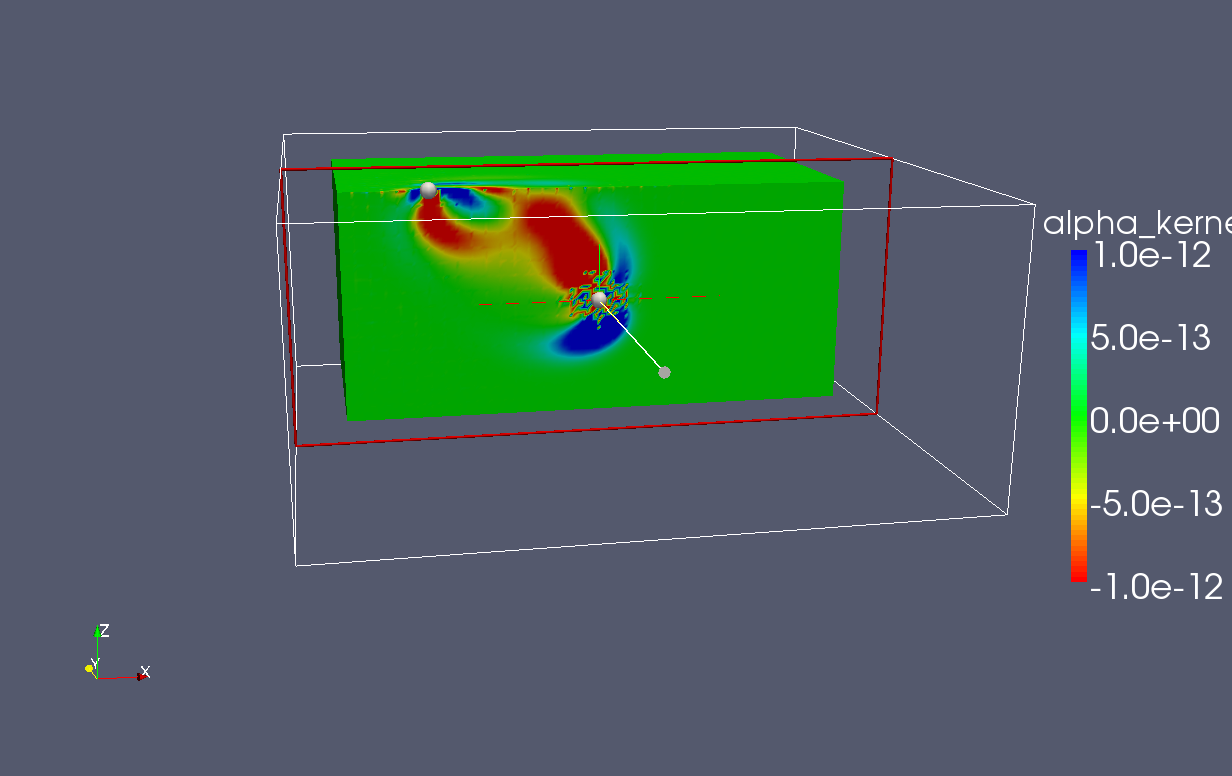
\includegraphics[width=0.7\textwidth]{homogeneous_halfspace_P_kernel.png}
\end{center}
\caption{$P$ travel-time sensitivity kernel for example 2}
\end{figure}

Note: The rescaling of the colour bar is necessary because the magnitude of the kernel is very large at the source and receiver locations due to the unrealistic assumption of point sources. To be able to distinguish the kernel itself, it is sometimes necessary to reduce the maximum values of the colour scale by four orders of magnitude. Smoothing these kernels to get rid of the spuriously large values at the sources and receivers is prudent before using them in tomographic inversions.
   
Again be sure to run \lstinline{module unload paraview PrgEnv-gnu} before proceeding to other examples.

\end{enumerate}

\blue{note that there are some new scripts added (by Daniel?)}


%===============================================================================

\subsection*{Step-by-step instructions, example 3: southern California}

This example is at a scale that will likely not run on a single laptop or desktop computer. In other words, the required memory must be distributed over a number of different machines in order to run the simulation. Here we use 96 cores of the cluster.

\begin{enumerate}
\item Copy bash scripts into the base directory:

\begin{lstlisting}
$ cd SPECFEM3D_socal
$ cp ../SPECFEM3D_default/*bash .
\end{lstlisting}

\item configure
\begin{lstlisting}
$ ./configure FC=pgf90 MPIFC=mpif90
\end{lstlisting}

\item compile all
\begin{lstlisting}
$ make all
\end{lstlisting}

\item Link the mesh directory as an example
\begin{lstlisting}
$ cd examples
$ ln -s /import/c/d/ERTHQUAK/GEOCUBIT_MESH/socal_med400km .
\end{lstlisting}

\item Modify \path{go_decomposer_pbs.bash} to point to the new directory:
\begin{lstlisting}
MESHDIR=examples/socal_med400km/MESH/
\end{lstlisting}

\item Link the tomography file and copy input files
\begin{lstlisting}
$ cd DATA
$ ln -s /import/c/d/ERTHQUAK/MODEL/cvm119_1000_1000_0250_741_549.xyz tomography_model.xyz
$ cp ../examples/socal_med400km/in_data_files/* .
\end{lstlisting}

\item modify \path{go_generate_databases_pbs.bash} and \path{go_solver_pbs.bash} to have the proper time limits and number of cores
\begin{lstlisting}
#PBS -l nodes=6:ppn=16,walltime=1:00:00
#PBS -q standard
\end{lstlisting}

%\item delete the empty directory
%
%\begin{lstlisting}
%rm -rf OUTPUT_FILES/DATABASES_MPI
%\end{lstlisting}
%
%This simulation will create a directory \path{DATABASES_socal_med400km} that is outside of \path{OUTPUT_FILES}. This is useful% since we may have many simulations associated with the same mesh.

\item Follow the same steps as in Example 1: decompose, generate databases, solver. Here the programs have all been compiled, so only submitting the run scripts is needed. (But wait for each one to finish, and check the output before proceeding to the next step.)
%
\begin{itemize}
\item The decomposer takes about 3 minutes.
\item The generate databases takes about 15 minutes.
\item The solver takes about 25 minutes.
\end{itemize}
%
The simulation runs on 96 cores and should take about 25 minutes. You can track the progress with the timestamp files generated in \path{OUTPUT_FILES/} (type \lstinline{ls -ltr} to see the most recent files). When the job is complete, you should have 3 sets (semd,semv,sema) of 1107 (\lstinline{ls -1 *semd | wc}) seismogram files in the directory \path{OUTPUT_FILES}, as well as 4 \path{timestamp******} files.

As expected, the seismograms contain numerical noise, since the source half duration in \path{CMTSOLUTION} was set to 0~s. This allows for maximal flexibility in post-processing, since the seismograms can be convolved with any source time function (see manual). However, it is important to know what the minimum resolving period of a particular mesh and model is, since these periods provide a guide for how to filter the seismograms in post-processing.

\item Now make a change to one of the input files in \path{SPECFEM3D/DATA/}, either \path{Par_file}, \path{CMTSOLUTION}, or \path{STATIONS}. Rename the \path{OUTPUT_FILES} directory if you do not want to over-write your previous output. Then submit the new job. (Note that no recompilation is needed.)

\end{enumerate}

%===============================================================================

\subsection*{Step-by-step instructions, example 4: GPU}

In this example, we show how \specfem\ can be used on a GPU cluster. In general,
there are only two {\em required} steps to use GPU computing:

\begin{enumerate}
\item Enable CUDA during configuration:
\begin{lstlisting}
$ ./configure --enable-cuda MPI_INC=-I$MPI_DIR/include
\end{lstlisting}

\item Enable CUDA at runtime in \path{DATA/Par_file}:
\begin{lstlisting}
GPU_MODE    =   .true.
\end{lstlisting}
\end{enumerate}

In practice, you may need to do several other steps depending on how your
cluster has been set up. When running on your own cluster, you should consult
their documentation in case there are additional steps that must be taken. The
following example shows the extra steps that are required on the FISH cluster
at ARSC.

\begin{enumerate}
\item *TODO*: start with login to fish

\item Check out version XXX again:
\begin{lstlisting}
$ git clone --recursive https://github.com/geodynamics/specfem3d.git SPECFEM3D_GPU
$ cd SPECFEM3D_GPU
\end{lstlisting}

\item Load the CUDA toolkit:
\begin{lstlisting}
$ module load cudatoolkit
\end{lstlisting}

\item The compilers on fish work a little differently than on pacman. There are
      wrappers that automatically run the real compilers and apply MPI or CUDA
      options once the modules are loaded.

      When compiling for CUDA, the CUDA compiler (which is separate from the C
      or Fortran compilers) needs to know where the MPI headers are installed.
      This information must be set using the \texttt{MPI\_INC} variable when
      running \path{./configure}. On fish, loading the MPI module sets the
      \texttt{MPICH\_DIR} environment variable, which is used in the instructions
      below.

\begin{lstlisting}
$ ./configure MPIFC=ftn CC=cc FC=ftn --with-cuda MPI_INC=-I$MPICH_DIR/include
\end{lstlisting}

\item *TODO*: Copy example config stuff...

\item The GPU mode only affects the solver (\path{xspecfem3D}), but it is a good
      idea to remember to enable it now. Edit \path{DATA/Par_file} and set this
      option:
\begin{lstlisting}
GPU_MODE    =   .true.
\end{lstlisting}

\item Now, you can compile things as usual:
\begin{lstlisting}
$ make xdecompose_mesh
$ make xgenerate_databases
$ make xspecfem3D
\end{lstlisting}

\item The scripts to run jobs on fish are similar to the ones on pacman. Fish
      uses a slightly different method to run MPI programs compared to pacman.
      Instead of using \lstinline{mpirun -np <#procs>}, you use
      \lstinline{aprun -n <#procs>}, and to use GPUs, you must use the \texttt{gpu}
      queue.
\begin{lstlisting}
$ cd utils/Cluster/pbs/
$ cp go_decomposer_pbs.bash go_generate_databases_pbs.bash go_solver_pbs.bash ../../../
$ cd ../../../
$ vim *.bash
  # Change 'mpirun -np' to 'aprun -n'
  # Change '#PBS -q standard' to '#PBS -q gpu' (only necessary for go_solver_pbs.bash)
\end{lstlisting}
*TODO*: Add note about one process per node for GPU runs. This probably depends
on which example we're using.

\item Now, you can submit your jobs as usual:
\begin{lstlisting}
$ qsub go_decomposer_pbs.bash
# Wait for it to finish

$ qsub go_generate_databases_pbs.bash
# Wait for it to finish

$ qsub go_solver_pbs.bash
# Wait for it to finish
\end{lstlisting}

\item Depending on how many GPUs you use, you may see up to 20 or 30 times
      faster execution. If everything ran correctly on the GPU, you should see
      some additional files in \path{OUTPUT_FILES}:
\begin{lstlisting}
$ ls OUTPUT_FILES/gpu*.txt
gpu_device_info_proc_000000.txt
gpu_device_mem_usage_proc_000000.txt
gpu_device_info_proc_000001.txt
gpu_device_mem_usage_proc_000001.txt
gpu_device_info_proc_000002.txt
gpu_device_mem_usage_proc_000002.txt
gpu_device_info_proc_000003.txt
gpu_device_mem_usage_proc_000003.txt
\end{lstlisting}

      These files contain statistics of the run on the GPU devices. If the jobs
      crash, you should check these files to ensure that you did not use too
      much memory per GPU.
\end{enumerate}

%=====================================================
% REFERENCES

%\begin{spacing}{1.0}
%\bibliographystyle{agu08}
%\bibliography{preamble,REFERENCES,refs_carl,refs_socal,refs_source}
%\end{spacing}

%=====================================================
\end{document}
%=====================================================
